\documentclass[20pt, a2paper, landscape]{tikzposter}
\usepackage{siunitx}
\usepackage{tabularx}

\title{QEA Boat}
\author{Kawin Nikomborirak, Amy Phung}
\date{\today}

\usetheme{Desert}
\begin{document}
\maketitle

\begin{columns}
  \column{0.4}

  \block{Best Of All Time}
  {
    \begin{tabularx}{0.4\textwidth}{l X}
    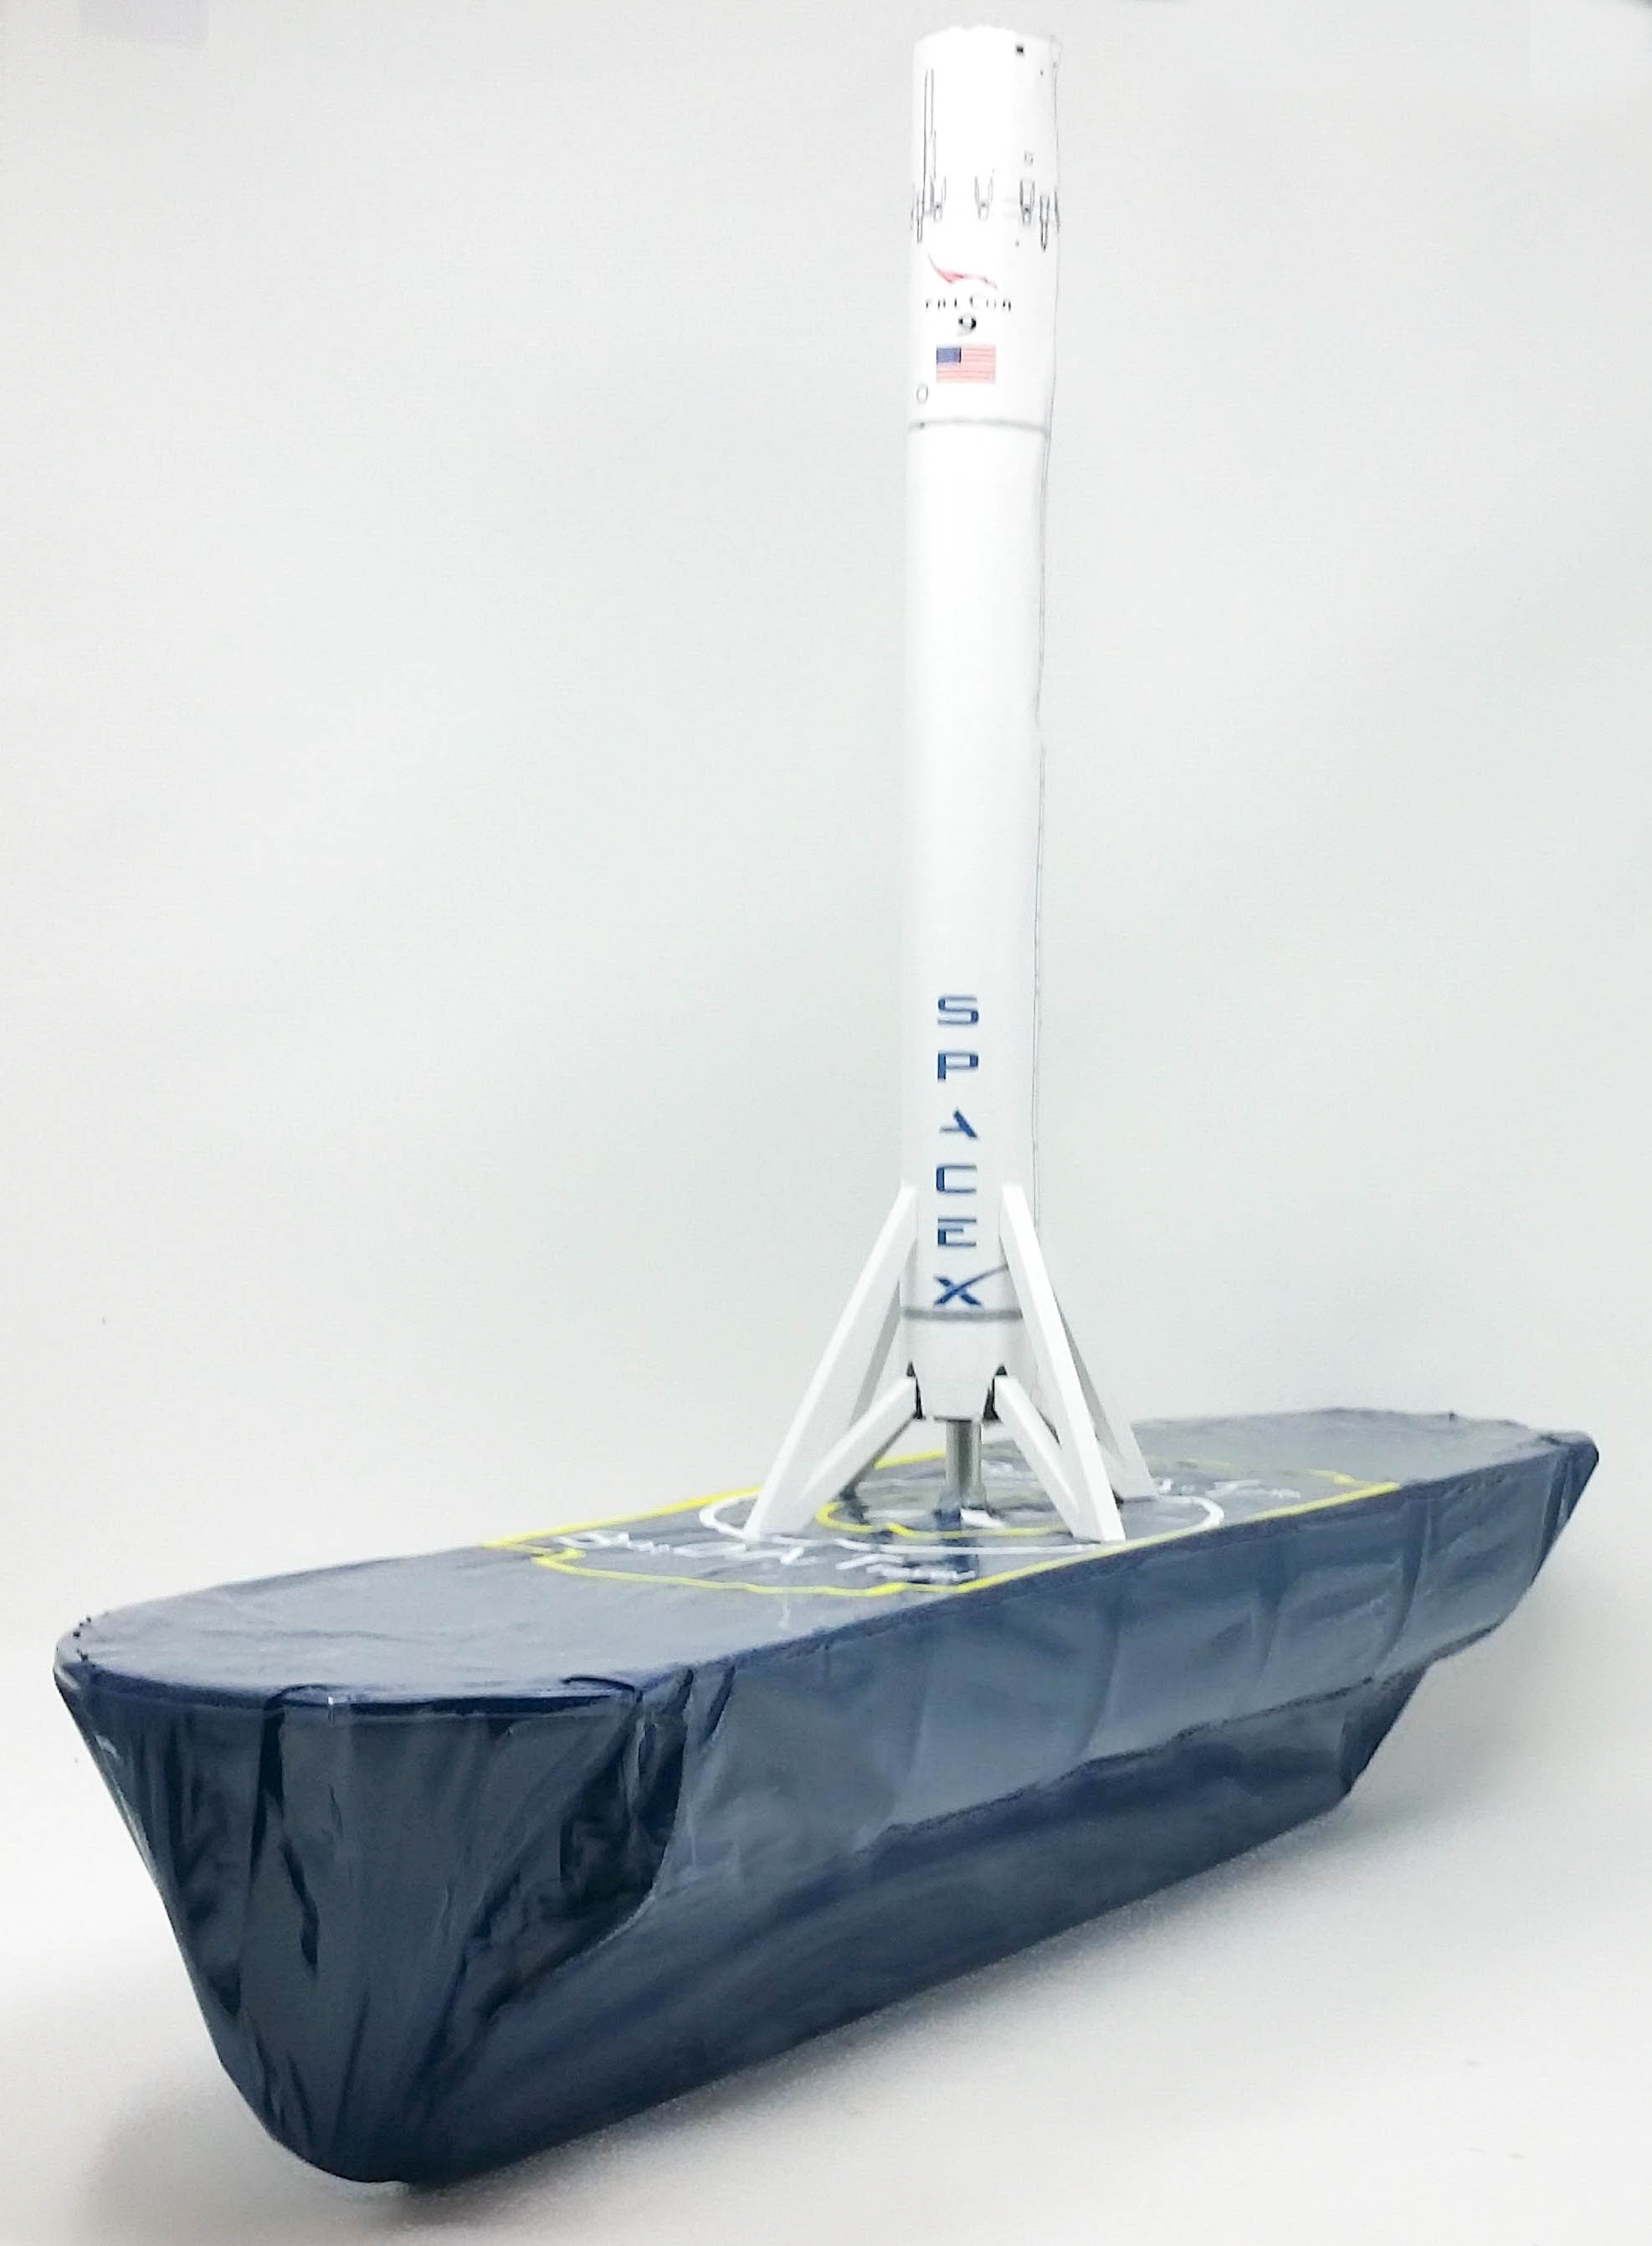
\includegraphics[width=0.17\textwidth]{FinishedBoat.jpg} &
    Boat of Air Transportation
    \end{tabularx}
  }

  \block{Performance Considerations}
  {
    \begin{itemize}
    \item The boat has a functional keel to lower COM.
    \item The AVS should be \ang{130}
    \item Minimize the wet surface friction
    \item The boat should be as long as possible
    \end{itemize}
  }


  \column{0.6}
  \block{Righting Moment vs Heel Angle}{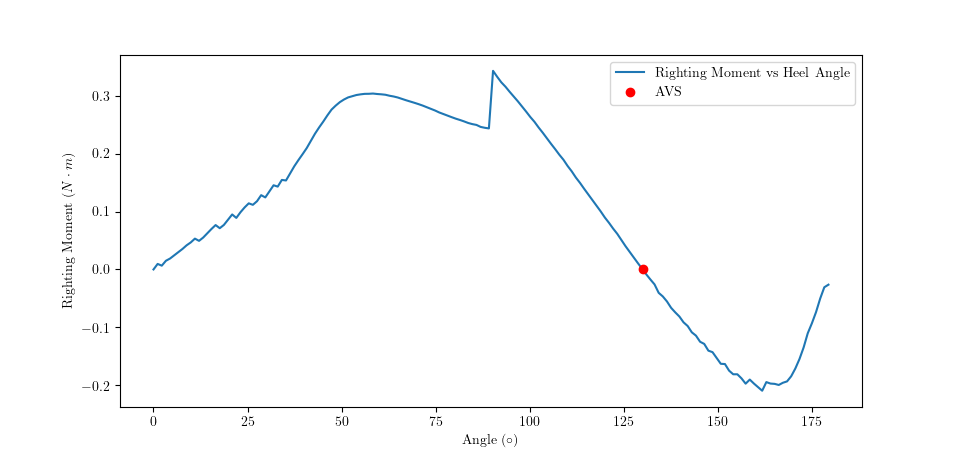
\includegraphics[width=0.53\textwidth]{curve.png}}

  \block{Performance of boats}
  {
    The boat in terms of floating level and AVS was right on the dot.
    The boat cruised at around \SI{.7}{\meter\per\second}; slow but faster than the SolidWorks simulation.
    The speed being faster than SolidWorks is due to the nature of fluid simulation, and the slow speed was due to wrinkles on the hull as well to a lot of wet surface area.
  }


\end{columns}

\end{document}
